\documentclass{article}
\usepackage{amsmath}
\usepackage{gvv-book}
\usepackage{float}
\usepackage{gvv}
\begin{document}
\begin{enumerate}
       \item let $f:R_{+} \rightarrow [-5, \infty)$ be defined as $f(x) = 9x^{2} +6x -5$ where $R_{+}$ is the set of all non-negative real numbers, then $f$ is:
	       \begin{enumerate}
		       \item one-one
		       \item onto
		       \item bijective
		       \item neither one-one nor onto
	       \end{enumerate}
       \item The number of points of discontinuity of $f(x) = \begin{dcases}
		       |x|+3, & if x\leq-3  \\
		       -2x, & if -3<x<3 \\
		       6x+2, & if x\geq3 
       \end{dcases}$ is:
		\begin{enumerate}
			\item $0$
			\item $1$
			\item $2$
			\item infinite
		\end{enumerate}
	\item The function $f(x) = x^{3} - 3x^{2} +12x -18$ is:
		\begin{enumerate}
			\item strictly decreasing on $R$
			\item strictly increasing on $R$
			\item neither strictly increasing nor strictly decreasing on $R$
			\item strictly decreasing on $(-\infty, 0)$
		\end{enumerate}
	\item Find the domain of the function $f(x) = \sin^{-1}(x^{2} - 4$. Also, find its range.
	\item If $f(x) = |\tan 2x|$, then find the value of $f'(x)$ at $x=\frac{\pi}{3}$.
	\item If $M$ and $m$ denote the local maximum and local minimum values of the function $f(x) = x + \frac{1}{x} (x\neq0)$ respectively, find the value of $(M-m)$.
	\item Show that $f(x) = e^{x} - e^{-x} + x - \tan^{-1}x$ is strictly increasing in its domain.
	\item Show that a function $f:R \rightarrow R$ defined bt $f(x) = \frac{2x}{1+x ^{2}}$ is neither one-one nor onto. Further, find set $A$ so that the given function $f:R \rightarrow A$ becomes an onto function.
	\item A relation $R$ is defined on $N \times N$ (where $N$ is the set f natural numbers) as:\\
		\centerline{$(a,b)R(c,d) \leftrightarrow a - c = b - d$}\\
	Show that $R$ is an equivalence relation.
        \item The month of September is celebrtaed as the Rashtriya Poshan Maah across the country. Following a healthy and well-balanced diet is crucial in order to supply the body with the proper nutrients it needs. A balanced diet also keeps us mentally fit and promotes improved level of energy.\\
		\begin{figure}[h]
			\centering 
			      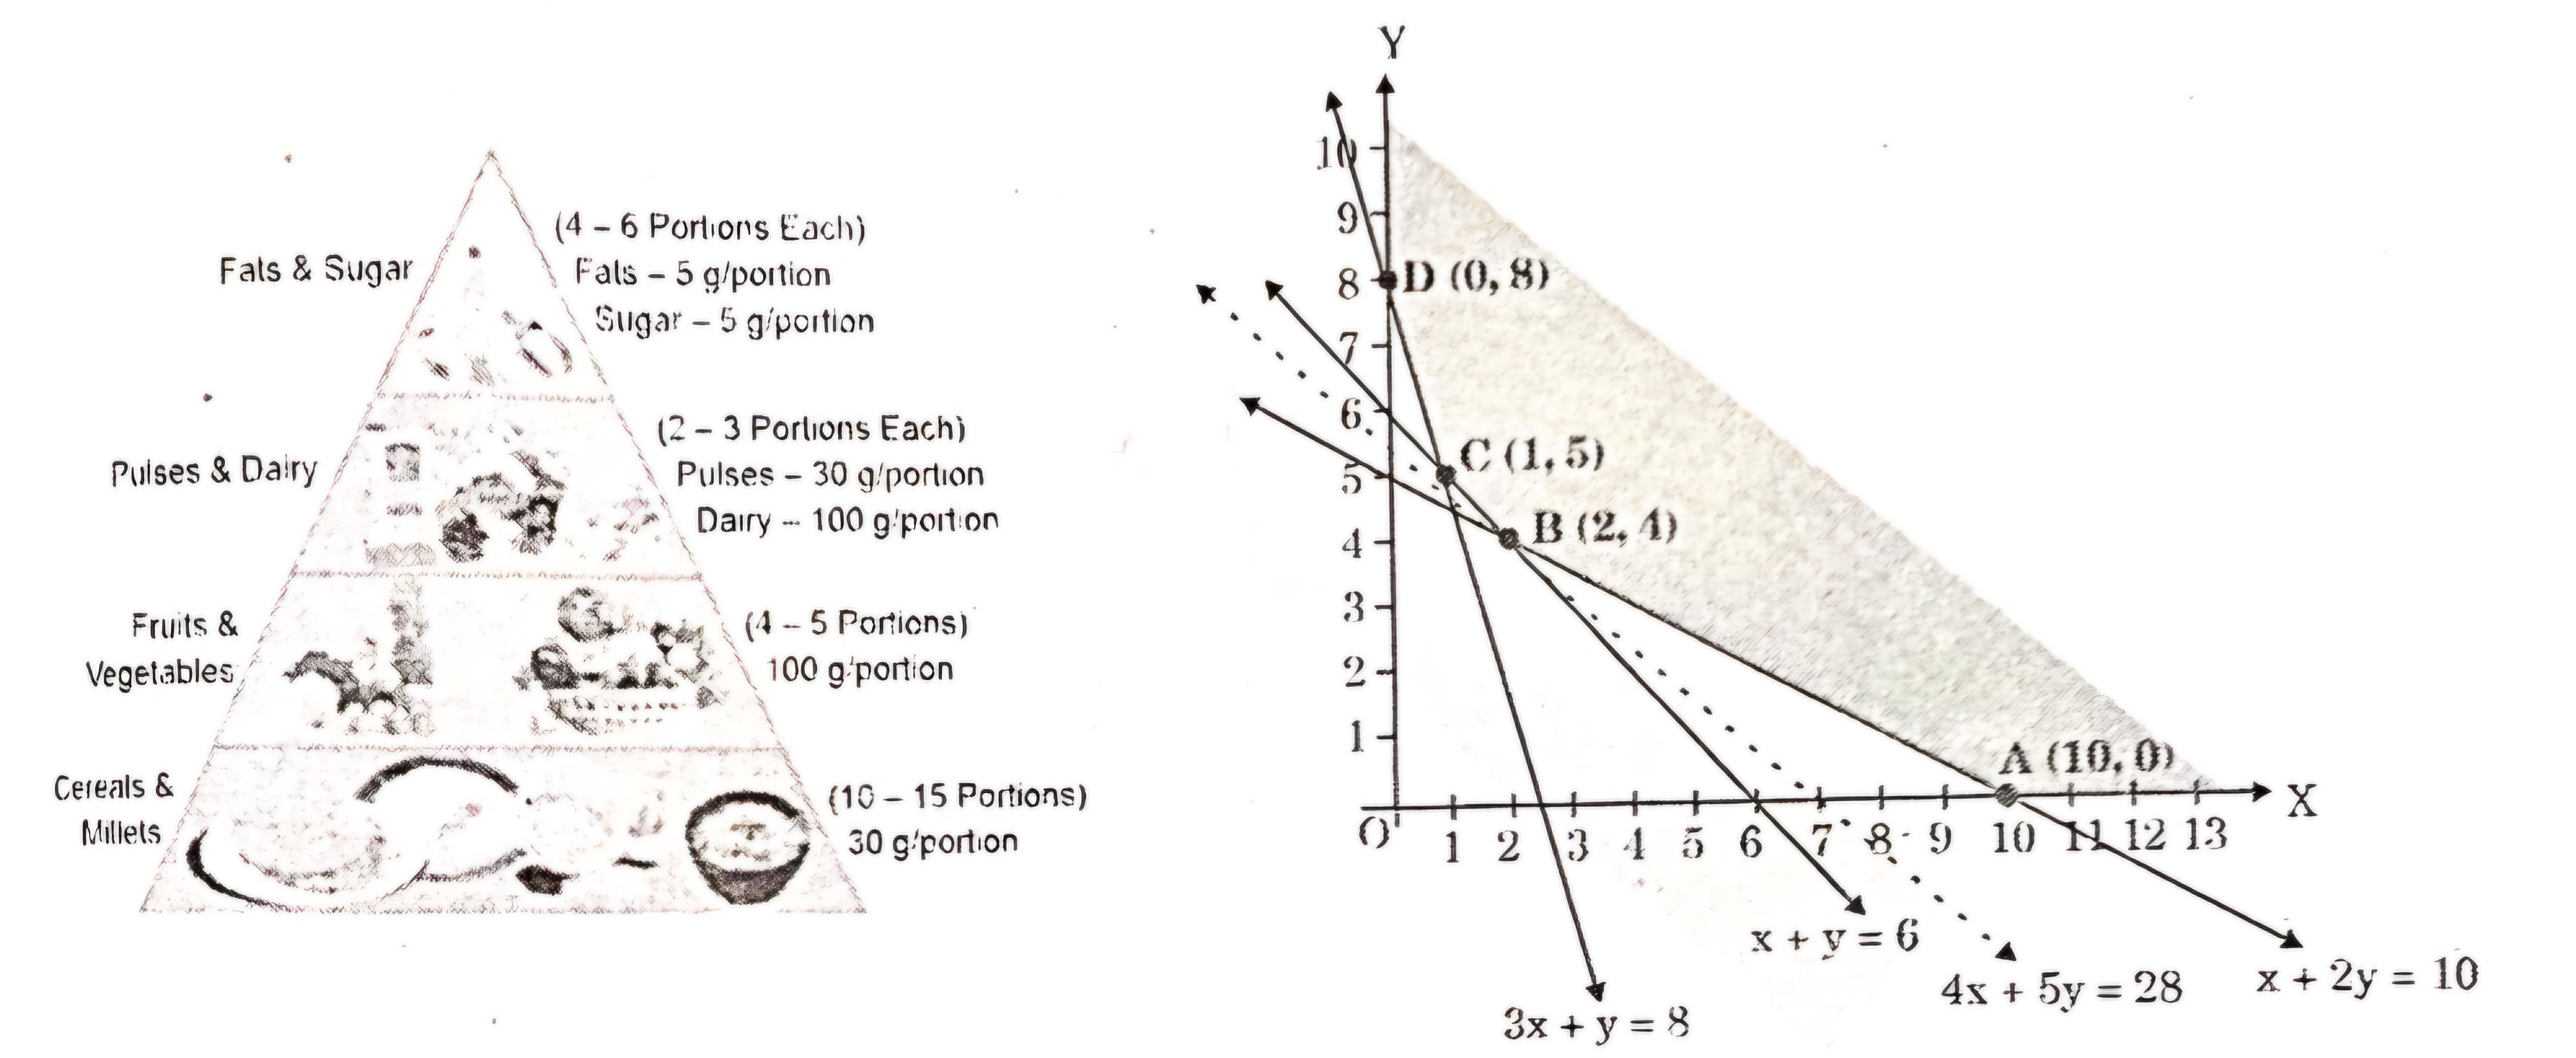
\includegraphics[width=120mm]{./Figuress/Graphs.jpg}
			      \caption{1}
			\label{figure}
		\end{figure}
		A dietician wishes to minimize the cost of a diet involving two types of foods,food $X (x kg)$ and fodd $Y (y kg)$ which are available at the rate of $\rupee 16/kg$ and $\rupee 20/kg$ respectively. The feasible region satisfying the constraints is shown in the graph.\\
		On the basis of the above information, answer the following questions:
		\begin{enumerate}[label=(\roman*)]
			\item Identify and write all the constraints which determine the given feasible region in the above graph.
			\item If the objective is to minimize cost $Z = 16x +20y$, find the values of $x$ and $y$ at which cost is minimum. Also, find minimum cost assuming that minimum cost is possiblr for the given unbounded region.
		\end{enumerate}
\end{enumerate}
\end{document}
